\documentclass{tufte-handout}
\usepackage{pgfplots}
\usepackage[dvipsnames]{xcolor}
\usepackage{amsmath, amssymb, amsthm}
\usepackage{mathtools}
\usepackage{bm}
\usepackage{thmtools}
\usepackage{enumitem}
\usepackage{algorithm}
\usepackage{algpseudocode}
\usepackage{tikz}
\usetikzlibrary{calc,arrows.meta,positioning}

\let\subsubsection\subsection

% Color scheme (matching your existing document)
\definecolor{wp-bg}{HTML}{FDF6EF}
\definecolor{wp-text}{HTML}{2D1B0E}
\definecolor{wp-primary}{HTML}{C24A3A}
\definecolor{wp-accent}{HTML}{D4952E}
\definecolor{wp-light}{HTML}{F0DECA}
\definecolor{wp-muted}{HTML}{C4A88A}
\definecolor{wp-dark}{HTML}{1A0F07}

\pagecolor{wp-bg}
\color{wp-text}
\hypersetup{colorlinks=true,linkcolor=wp-primary,urlcolor=wp-accent}

% Theorem environments
\declaretheorem[style=plain, name=Definition, numberwithin=section]{defn}
\declaretheorem[style=plain, name=Theorem, numberwithin=section]{thm}
\declaretheorem[style=plain, name=Lemma, numberwithin=section]{lem}
\declaretheorem[style=remark, name=Example, numberwithin=section]{exmp}
\declaretheorem[style=remark, name=Remark, numberwithin=section]{remark}

\title{Recurrent Neural Networks \\ Mathematical Foundations}
\author{Vitor N. Cabral de Oliveira\\ \href{mailto:vnco@cin.ufpe.br}{vnco@cin.ufpe.br}}
\date{\today}

\begin{document}

\maketitle

\begin{abstract}
    This chapter develops the mathematical framework for Recurrent Neural Networks (RNNs), which are designed to process sequential data. We formalise the RNN architecture, derive the forward propagation equations, and present backpropagation through time (BPTT). The problems of vanishing and exploding gradients are analysed, and the Long Short‑Term Memory (LSTM) and Gated Recurrent Unit (GRU) are introduced as effective solutions.
\end{abstract}

\newpage
\hypersetup{linkcolor=wp-text}
\tableofcontents
\hypersetup{linkcolor=wp-primary}
\newpage


\section{Foundations of Sequence Modeling}

Before diving into recurrent architectures, we must establish a rigorous framework for sequence data. Sequences are ordered collections of observations that arise naturally in time series, natural language, audio, video, and many other domains. Understanding their structure and the associated learning problems is essential.

\subsection{Definition and Notation}

\begin{defn}[Sequence]
    A \textbf{sequence} of length $T$ is an ordered tuple $\mathbf{x}_{1:T} = (\mathbf{x}_1, \mathbf{x}_2, \dots, \mathbf{x}_T)$, where each element $\mathbf{x}_t$ belongs to a set $\mathcal{X}$ (the \textbf{observation space}). When $\mathcal{X} \subseteq \mathbb{R}^d$, we speak of a \textbf{real‑valued vector sequence}. 
    \begin{itemize}
        \item If $T$ is finite, the sequence is \textbf{finite}; if $T = \infty$, it is \textbf{infinite}.
        \item When the indices $t$ are discrete (e.g., $t \in \mathbb{N}$), we have a \textbf{discrete‑time sequence}. Continuous‑time sequences are indexed by $t \in \mathbb{R}$ but are less common in machine learning.
    \end{itemize}
\end{defn}

\begin{marginfigure}
\centering
\begin{tikzpicture}[scale=0.8]
    \begin{axis}[width=4cm, height=2.5cm, xlabel=$t$, ylabel=$x_t$, domain=0:10, samples=100, axis lines=middle, enlargelimits]
        \addplot[wp-primary, thick] {sin(deg(x)) + 0.2*rand};
    \end{axis}
    \caption{A real‑valued discrete‑time sequence (time series).}
\end{tikzpicture}
\end{marginfigure}

\paragraph{Special cases}
\begin{itemize}
    \item \textbf{Univariate sequence}: each $\mathbf{x}_t \in \mathbb{R}$ (scalar). Example: daily temperature.
    \item \textbf{Multivariate sequence}: each $\mathbf{x}_t \in \mathbb{R}^d$, $d>1$. Example: joint angles of a robotic arm over time.
    \item \textbf{Symbolic sequence}: $\mathcal{X}$ is a finite set of symbols (e.g., characters, words). Example: natural language text.
\end{itemize}

\subsection{Probabilistic Description}

A sequence can be modelled as a \textbf{stochastic process} $\{X_t\}_{t \in \mathcal{T}}$, where each $X_t$ is a random variable taking values in $\mathcal{X}$, and $\mathcal{T}$ is the index set (usually $\mathbb{N}$ or $\{1,\dots,T\}$). The joint distribution over the entire sequence is $P(X_1 = x_1, \dots, X_T = x_T)$.

\begin{defn}[Stationarity]
    A stochastic process is \textbf{strictly stationary} if for any $t_1,\dots,t_k$ and any shift $\tau$,
    \[
    P(X_{t_1} \le x_1, \dots, X_{t_k} \le x_k) = P(X_{t_1+\tau} \le x_1, \dots, X_{t_k+\tau} \le x_k).
    \]
    It is \textbf{weakly stationary} (or covariance stationary) if:
    \begin{enumerate}
        \item $\mathbb{E}[X_t] = \mu$ (constant mean),
        \item $\operatorname{Var}(X_t) = \sigma^2$ (constant variance),
        \item $\operatorname{Cov}(X_t, X_{t+\tau})$ depends only on $\tau$ (the lag).
    \end{enumerate}
\end{defn}

Stationarity simplifies modeling because the statistical properties do not change over time. Many real‑world sequences are non‑stationary (e.g., financial returns have time‑varying volatility).

\subsection{Auto‑correlation and Memory}

A key characteristic of sequences is that observations are not independent; they exhibit \textbf{temporal dependence}.

\begin{defn}[Auto‑correlation Function (ACF)]
    For a weakly stationary sequence with variance $\sigma^2$, the auto‑correlation at lag $\tau$ is
    \[
    \rho(\tau) = \frac{\operatorname{Cov}(X_t, X_{t+\tau})}{\sigma^2}.
    \]
    The ACF satisfies $\rho(0)=1$, $|\rho(\tau)|\le 1$, and $\rho(\tau)=\rho(-\tau)$.
\end{defn}

If $\rho(\tau)$ decays slowly (e.g., $\rho(\tau) \sim e^{-\alpha \tau}$ or power‑law), the sequence has \textbf{long‑term memory}. Short‑memory processes have $\rho(\tau) \to 0$ exponentially fast.

\begin{marginfigure}
\centering
\begin{tikzpicture}[scale=0.7]
    \begin{axis}[width=4cm, height=2.5cm, xlabel=$\tau$, ylabel=$\rho(\tau)$, domain=0:10, samples=50, axis lines=middle, enlargelimits]
        \addplot[wp-primary, thick] {exp(-0.5*x)};
        \addplot[wp-accent, thick] {0.8^abs(x)};
        \legend{fast decay, slow decay};
    \end{axis}
    \caption{Auto‑correlation functions: exponential (fast) vs. power‑law (slow).}
\end{tikzpicture}
\end{marginfigure}

\subsection{Markov Property and Order}

A fundamental simplification for sequence modeling is the Markov assumption: the future depends only on a finite past.

\begin{defn}[Markov Chain]
    A discrete‑time stochastic process $\{X_t\}$ is a \textbf{Markov chain of order $k$} if for all $t$,
    \[
    P(X_t = x_t \mid X_{1:t-1} = x_{1:t-1}) = P(X_t = x_t \mid X_{t-k:t-1} = x_{t-k:t-1}),
    \]
    i.e., the conditional distribution of the next state depends only on the $k$ most recent states. For $k=1$, it is a \textbf{first‑order Markov chain}.
\end{defn}

\begin{thm}[Markov Chain Decomposition]
    For a first‑order Markov chain, the joint distribution factorizes as
    \[
    P(X_{1:T} = x_{1:T}) = P(X_1 = x_1) \prod_{t=2}^{T} P(X_t = x_t \mid X_{t-1} = x_{t-1}).
    \]
\end{thm}

The Markov property is the theoretical backbone of many sequence models, including RNNs (which approximate an infinite‑order Markov chain via hidden states).

\subsection{Sequence Learning Tasks}

We categorise learning problems based on inputs and outputs:

\begin{enumerate}
    \item \textbf{Sequence prediction (auto‑regressive)}: Given past observations $x_{1:t-1}$, predict $x_t$. The model learns $P(x_t \mid x_{1:t-1})$.
    \item \textbf{Sequence classification}: Given the entire input sequence $\mathbf{x}_{1:T}$, predict a single label $y$. Example: sentiment analysis.
    \item \textbf{Sequence labelling (per‑time‑step classification)}: Given $\mathbf{x}_{1:T}$, predict a label $y_t$ for each $t$. Example: part‑of‑speech tagging.
    \item \textbf{Sequence generation}: Sample a new sequence from the learned distribution $P(x_{1:T})$.
    \item \textbf{Sequence‑to‑sequence (seq2seq)}: Map an input sequence $\mathbf{x}_{1:T}$ to an output sequence $\mathbf{y}_{1:T'}$ (possibly of different length). Example: machine translation.
\end{enumerate}

\subsection{Why Feedforward Networks Fail for Sequences}

Feedforward (multilayer perceptron) networks assume fixed‑length inputs and outputs, and – critically – they treat each input as independent. To process a sequence of length $T$, one could:
\begin{enumerate}
    \item \textbf{Concatenate all elements} into a single $d \times T$ vector. This fails because $T$ is variable and the resulting dimension becomes enormous.
    \item \textbf{Slide a window} of fixed size $w$ over the sequence, using the last $w$ values as input to a feedforward network. This ignores dependencies longer than $w$ (finite memory) and does not share parameters across time positions efficiently.
\end{enumerate}

Moreover, feedforward networks have no built‑in mechanism to handle the sequential order or to maintain a state that evolves over time. They cannot capture the inductive bias that the same transformation applies at each time step (weight sharing) – a property that recurrent networks exploit.

\begin{marginfigure}
\centering
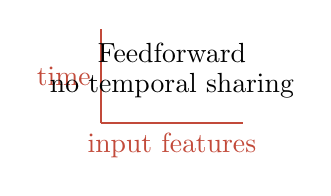
\begin{tikzpicture}[scale=0.6]
    \draw[thick, wp-primary] (0,0) -- (0,2) node[midway, left] {time};
    \draw[thick, wp-primary] (0,0) -- (3,0) node[midway, below] {input features};
    \node at (1.5,1.5) {Feedforward};
    \node at (1.5,0.8) {no temporal sharing};
\end{tikzpicture}
\caption{Feedforward networks treat each time step independently; they cannot share weights across time or maintain a dynamic state.}
\end{marginfigure}

\subsection{Recurrence as a Natural Solution}

An RNN addresses these limitations by introducing a \textbf{hidden state} $\mathbf{h}_t$ that evolves over time according to
\[
\mathbf{h}_t = f(\mathbf{h}_{t-1}, \mathbf{x}_t; \boldsymbol{\theta}),
\]
where $f$ is a parameterised function (same at each step). This gives three crucial properties:
\begin{itemize}
    \item \textbf{Variable‑length handling}: the same recurrence applies for any $T$.
    \item \textbf{Parameter sharing}: the same weights $\boldsymbol{\theta}$ are used at each time step, reducing the number of parameters and promoting generalization.
    \item \textbf{Memory}: the hidden state $\mathbf{h}_t$ can theoretically retain information from arbitrarily distant past (though in practice limited by vanishing gradients).
\end{itemize}

Thus, the RNN is a natural and principled extension of feedforward networks to sequential data. The remainder of this chapter formalises the RNN architecture, training, and its advanced variants.

\subsection{Further Reading}

For a deeper treatment of stochastic processes and sequence modeling, see:
\begin{itemize}
    \item Box, G. E. P., Jenkins, G. M., \& Reinsel, G. C. (2015). \textit{Time Series Analysis: Forecasting and Control}.
    \item Bishop, C. M. (2006). \textit{Pattern Recognition and Machine Learning} (Chapter 13: Sequential Data).
    \item Murphy, K. P. (2012). \textit{Machine Learning: A Probabilistic Perspective} (Chapter 17: Markov and Hidden Markov Models).
\end{itemize}

\subsection{Markov Models: From Chains to Hidden States}

The Markov property provides a powerful simplification for sequence modeling: the future depends only on a finite past. This idea gives rise to a family of models that are both mathematically tractable and widely used.

\subsubsection{Discrete‑Time Markov Chains}

\begin{defn}[Markov Chain – First Order]
    A discrete‑time stochastic process $\{X_t\}_{t=1}^\infty$ with state space $\mathcal{S}$ (finite or countable) is a \textbf{Markov chain} if for all $t \ge 2$ and all $s_1,\dots,s_t \in \mathcal{S}$,
    \[
    P(X_t = s_t \mid X_{t-1}=s_{t-1}, \dots, X_1=s_1) = P(X_t = s_t \mid X_{t-1}=s_{t-1}).
    \]
    The chain is \textbf{time‑homogeneous} if the transition probability does not depend on $t$:
    \[
    P(X_t = j \mid X_{t-1}=i) = T_{ij}, \quad \forall t,
    \]
    where $\mathbf{T}$ is the \textbf{transition matrix} with rows summing to $1$.
\end{defn}

\begin{marginfigure}
\centering
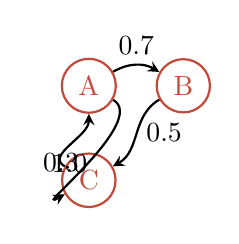
\begin{tikzpicture}[node distance=1.2cm, thick, >=stealth]
    \node[draw, circle, wp-primary] (A) {A};
    \node[draw, circle, wp-primary, right of=A] (B) {B};
    \node[draw, circle, wp-primary, below of=A] (C) {C};
    \draw[->] (A) to[out=30,in=150] node[above] {$0.7$} (B);
    \draw[->] (A) to[out=-30,in=-150] node[left] {$0.3$} (C);
    \draw[->] (B) to[out=210,in=30] node[right] {$0.5$} (C);
    \draw[->] (C) to[out=150,in=-90] node[below] {$1.0$} (A);
\end{tikzpicture}
\caption{A three‑state Markov chain with transition probabilities.}
\end{marginfigure}

\begin{defn}[Order $k$ Markov Chain]
    A process satisfies the \textbf{Markov property of order $k$} if
    \[
    P(X_t \mid X_{1:t-1}) = P(X_t \mid X_{t-k:t-1}).
    \]
    The state can be augmented to $\tilde{X}_t = (X_{t-k+1}, \dots, X_t)$, which forms a first‑order chain on a larger state space of size $|\mathcal{S}|^k$.
\end{defn}

\paragraph{Key Properties of Markov Chains}

\begin{itemize}
    \item \textbf{Stationary distribution}: If a distribution $\boldsymbol{\pi}$ satisfies $\boldsymbol{\pi}^{\mathsf{T}} = \boldsymbol{\pi}^{\mathsf{T}} \mathbf{T}$, it is stationary; for an ergodic chain, $\lim_{n\to\infty} \mathbf{T}^n$ has rows equal to $\boldsymbol{\pi}$.
    \item \textbf{Ergodicity}: A chain that is aperiodic and positive recurrent converges to a unique stationary distribution regardless of initial state.
    \item \textbf{Likelihood of a sequence}: $P(X_{1:T}=s_{1:T}) = P(X_1=s_1) \prod_{t=2}^T T_{s_{t-1}, s_t}$.
\end{itemize}

\subsubsection{Hidden Markov Models (HMMs)}

In many real‑world sequences, the underlying state is not directly observable. HMMs extend Markov chains by assuming that each state $X_t$ emits an observation $O_t$ through a known emission distribution.

\begin{defn}[Hidden Markov Model]
    An HMM is a doubly stochastic process $(X_t, O_t)_{t=1}^T$ where:
    \begin{enumerate}
        \item $\{X_t\}$ is a time‑homogeneous Markov chain with state space $\mathcal{S}$, initial distribution $\boldsymbol{\pi}$, and transition matrix $\mathbf{T}$.
        \item Given $X_t$, the observation $O_t$ is independent of all other states and observations, with emission probability $E(o \mid X_t=s) = P(O_t=o \mid X_t=s)$.
    \end{enumerate}
    The joint distribution of a sequence of states and observations is
    \[
    P(X_{1:T}=s_{1:T}, O_{1:T}=o_{1:T}) = \pi_{s_1} \prod_{t=2}^T T_{s_{t-1}, s_t} \prod_{t=1}^T E(o_t \mid s_t).
    \]
\end{defn}

\begin{marginfigure}
\centering
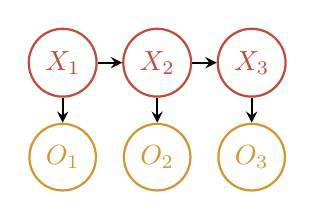
\begin{tikzpicture}[node distance=1.2cm, thick, >=stealth]
    \node[draw, circle, wp-primary] (X1) {$X_1$};
    \node[draw, circle, wp-primary, right of=X1] (X2) {$X_2$};
    \node[draw, circle, wp-primary, right of=X2] (X3) {$X_3$};
    \draw[->] (X1) -- (X2);
    \draw[->] (X2) -- (X3);
    \node[draw, circle, wp-accent, below of=X1] (O1) {$O_1$};
    \node[draw, circle, wp-accent, below of=X2] (O2) {$O_2$};
    \node[draw, circle, wp-accent, below of=X3] (O3) {$O_3$};
    \draw[->] (X1) -- (O1);
    \draw[->] (X2) -- (O2);
    \draw[->] (X3) -- (O3);
\end{tikzpicture}
\caption{Graphical model of an HMM: hidden states $X_t$ (circle) emit observations $O_t$ (square).}
\end{marginfigure}

\subsubsection{Inference and Learning in HMMs}

Three fundamental problems for HMMs are solved with efficient dynamic programming algorithms.

\paragraph{1. Likelihood Computation (Forward Algorithm)}
Given observations $o_{1:T}$, compute $P(O_{1:T}=o_{1:T}) = \sum_{s_{1:T}} P(X_{1:T}, O_{1:T})$. The forward recursion:
\[
\alpha_1(s) = \pi_s \, E(o_1 \mid s), \quad
\alpha_t(s) = E(o_t \mid s) \sum_{s'} \alpha_{t-1}(s') \, T_{s', s}.
\]
Then $P(O_{1:T}) = \sum_s \alpha_T(s)$.

\paragraph{2. Most Likely State Sequence (Viterbi)}
Find $\arg\max_{s_{1:T}} P(X_{1:T} \mid O_{1:T})$. The Viterbi algorithm uses:
\[
\delta_1(s) = \pi_s E(o_1 \mid s),\quad
\delta_t(s) = E(o_t \mid s) \max_{s'} \delta_{t-1}(s') T_{s', s},
\]
with backpointers to reconstruct the optimal path.

\paragraph{3. Parameter Estimation (Baum–Welch / EM)}
Given observations but no states, we maximise $\log P(O_{1:T} \mid \boldsymbol{\theta})$ via the EM algorithm. The E‑step computes posterior probabilities $\gamma_t(s) = P(X_t=s \mid O_{1:T})$ and $\xi_t(s',s) = P(X_{t-1}=s', X_t=s \mid O_{1:T})$ using the forward–backward algorithm. The M‑step updates:
\[
\pi_s \propto \gamma_1(s),\quad T_{s',s} \propto \frac{\sum_{t=2}^T \xi_t(s',s)}{\sum_{t=2}^T \gamma_{t-1}(s')},\quad
E(o \mid s) \propto \frac{\sum_{t: O_t=o} \gamma_t(s)}{\sum_t \gamma_t(s)}.
\]

\begin{thm}[Baum–Welch Convergence]
    The Baum–Welch algorithm monotonically increases the likelihood $P(O_{1:T} \mid \boldsymbol{\theta})$ and converges to a local maximum of the likelihood.
\end{thm}

\subsubsection{Markov Decision Processes (MDPs) – A Brief Mention}

When actions influence state transitions, we obtain an MDP. While not purely generative, MDPs are foundational for reinforcement learning. An MDP is a tuple $(\mathcal{S}, \mathcal{A}, \mathcal{T}, \mathcal{R}, \gamma)$ where:
\begin{itemize}
    \item $\mathcal{S}$: state space,
    \item $\mathcal{A}$: action space,
    \item $\mathcal{T}(s' \mid s, a)$: transition probability,
    \item $\mathcal{R}(s,a)$: immediate reward,
    \item $\gamma \in [0,1]$: discount factor.
\end{itemize}
The goal is to find a policy $\pi(a \mid s)$ that maximises expected cumulative reward.

\subsubsection{From Hidden Markov Models to Recurrent Neural Networks}

HMMs and RNNs both address sequence modeling but differ fundamentally:

\begin{itemize}
    \item \textbf{State representation}: HMM states are discrete (finite $\mathcal{S}$); RNN states are continuous vectors $\mathbf{h}_t \in \mathbb{R}^{d_h}$. Continuous states allow exponentially more expressive power for a fixed dimensionality.
    \item \textbf{Transition function}: HMM transitions are linear (matrix multiplication on a simplex); RNN transitions are nonlinear (e.g., $\tanh(\mathbf{W}_{hh}\mathbf{h}_{t-1} + \mathbf{W}_{xh}\mathbf{x}_t)$), enabling the modelling of complex dynamics.
    \item \textbf{Emission model}: HMM emissions factorize as $E(o_t \mid s_t)$; RNNs can produce outputs that depend on the entire history via $\mathbf{h}_t$.
    \item \textbf{Learning}: HMMs are trained with EM (Baum–Welch), which guarantees local likelihood increase; RNNs use BPTT and stochastic gradient descent, which scale better to large state spaces and long sequences.
    \item \textbf{Long‑range dependencies}: HMMs suffer from exponentially many states to represent $k$‑th order dependencies; RNNs attempt to compress history into a fixed‑size vector (though suffer from vanishing gradients).
\end{itemize}

\begin{thm}[HMM as a Linear RNN]
    If the state vector $\mathbf{h}_t$ is taken as the vector of probabilities $P(X_t=s \mid \text{history})$, then the update $\mathbf{h}_t \propto \mathbf{E}_{o_t} \odot (\mathbf{T}^{\mathsf{T}} \mathbf{h}_{t-1})$ (normalised) is a linear recurrence (with a non‑linear normalisation). This is equivalent to the forward algorithm of an HMM.
\end{thm}

The inadequacies of HMMs for large‑scale sequence modeling – discrete state, linear transitions, independence of observations given state – motivated the development of more powerful models, including conditional random fields (CRFs) and ultimately recurrent neural networks. However, HMMs remain important for their interpretability, small‑sample efficiency, and theoretical guarantees.

\begin{marginfigure}
\centering
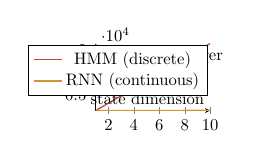
\begin{tikzpicture}[scale=0.6]
    \begin{axis}[width=4cm, height=3cm, xlabel=state dimension, ylabel=expressive power, domain=1:10, samples=2, axis lines=middle]
        \addplot[wp-primary, thick] {exp(x)};
        \addplot[wp-accent, thick] {1.5^x};
        \legend{HMM (discrete), RNN (continuous)};
    \end{axis}
\end{tikzpicture}
\caption{Continuous RNN states can represent exponentially more distinct histories than discrete HMM states of the same dimension.}
\end{marginfigure}



\section{Sequence Modeling and the Need for Recurrence}

Many machine learning tasks involve sequential data: time series, natural language text, audio signals, or video frames. In such data, each element depends not only on the current input but also on the history of previous elements. Standard feedforward networks (multilayer perceptrons) assume that inputs are independent, which fails for sequences.

A natural approach is to allow the network to maintain an internal \textbf{state} that evolves as it processes the sequence. This state serves as a memory that captures relevant information from the past. Recurrent Neural Networks (RNNs) are the canonical architecture for this purpose.

\begin{marginfigure}
\centering
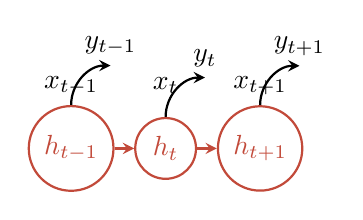
\begin{tikzpicture}[node distance=1.2cm, thick, >=stealth]
    \node[draw, circle, wp-primary] (h0) {$h_{t-1}$};
    \node[draw, circle, wp-primary, right of=h0] (h1) {$h_t$};
    \node[draw, circle, wp-primary, right of=h1] (h2) {$h_{t+1}$};
    \draw[->, wp-primary] (h0) -- (h1);
    \draw[->, wp-primary] (h1) -- (h2);
    \node[above of=h0, node distance=0.8cm] {$x_{t-1}$};
    \node[above of=h1, node distance=0.8cm] {$x_t$};
    \node[above of=h2, node distance=0.8cm] {$x_{t+1}$};
    \draw[->] (h0.north) to[out=90,in=180] ++(0.5,0.5) node[above] {$y_{t-1}$};
    \draw[->] (h1.north) to[out=90,in=180] ++(0.5,0.5) node[above] {$y_t$};
    \draw[->] (h2.north) to[out=90,in=180] ++(0.5,0.5) node[above] {$y_{t+1}$};
\end{tikzpicture}
\caption{Unrolled RNN: the same recurrent cell is applied at each time step, sharing weights across time.}
\end{marginfigure}

\subsection{Notation for Sequences}

Let a sequence be denoted by $\mathbf{x}_{1:T} = (\mathbf{x}_1, \mathbf{x}_2, \dots, \mathbf{x}_T)$, where each $\mathbf{x}_t \in \mathbb{R}^{d_x}$ is the input at time step $t$. The corresponding targets (if supervised) are $\mathbf{y}_{1:T} = (\mathbf{y}_1, \dots, \mathbf{y}_T)$ with $\mathbf{y}_t \in \mathbb{R}^{d_y}$ (or categorical). In many applications, the target at time $t$ depends on the entire history up to $t$.

\section{The Elman RNN Architecture}

The most basic RNN, proposed by Elman (1990), consists of an input layer, a hidden layer with recurrent connections, and an output layer. At each time step $t$, the hidden state $\mathbf{h}_t \in \mathbb{R}^{d_h}$ is updated based on the current input $\mathbf{x}_t$ and the previous hidden state $\mathbf{h}_{t-1}$.

\begin{defn}[RNN Cell]
    A simple RNN cell is defined by the following equations:
    \begin{align}
        \mathbf{a}_t &= \mathbf{W}_{xh} \mathbf{x}_t + \mathbf{W}_{hh} \mathbf{h}_{t-1} + \mathbf{b}_h, \label{eq:rnn_pre} \\
        \mathbf{h}_t &= \phi_h(\mathbf{a}_t), \label{eq:rnn_hidden} \\
        \mathbf{o}_t &= \mathbf{W}_{hy} \mathbf{h}_t + \mathbf{b}_y, \label{eq:rnn_output} \\
        \hat{\mathbf{y}}_t &= \phi_y(\mathbf{o}_t), \label{eq:rnn_pred}
    \end{align}
    where:
    \begin{itemize}
        \item $\mathbf{W}_{xh} \in \mathbb{R}^{d_h \times d_x}$ is the input‑to‑hidden weight matrix,
        \item $\mathbf{W}_{hh} \in \mathbb{R}^{d_h \times d_h}$ is the recurrent (hidden‑to‑hidden) weight matrix,
        \item $\mathbf{W}_{hy} \in \mathbb{R}^{d_y \times d_h}$ is the hidden‑to‑output weight matrix,
        \item $\mathbf{b}_h \in \mathbb{R}^{d_h}$, $\mathbf{b}_y \in \mathbb{R}^{d_y}$ are bias vectors,
        \item $\phi_h$ is a nonlinear activation function (typically $\tanh$ or ReLU),
        \item $\phi_y$ is the output activation (e.g., softmax for classification, identity for regression).
    \end{itemize}
    The initial hidden state $\mathbf{h}_0$ is usually set to the zero vector, but can also be learned.
\end{defn}

\begin{marginfigure}
\centering
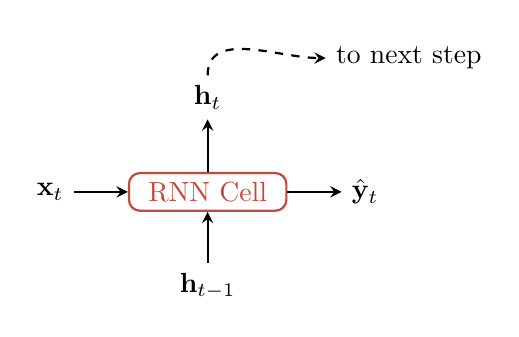
\begin{tikzpicture}[node distance=1cm, thick, >=stealth]
    \node[draw, rectangle, rounded corners, wp-primary, minimum width=2cm] (cell) {RNN Cell};
    \node[left of=cell, node distance=2cm] (x) {$\mathbf{x}_t$};
    \node[below of=cell, node distance=1.2cm] (hprev) {$\mathbf{h}_{t-1}$};
    \node[right of=cell, node distance=2cm] (y) {$\hat{\mathbf{y}}_t$};
    \node[above of=cell, node distance=1.2cm] (h) {$\mathbf{h}_t$};
    \draw[->] (x) -- (cell);
    \draw[->] (hprev) -- (cell);
    \draw[->] (cell) -- (y);
    \draw[->] (cell) -- (h);
    \draw[->, dashed] (h) to[out=90,in=180] ++(1.5,0.5) node[right] {to next step};
\end{tikzpicture}
\caption{Schematic of a single RNN cell. The hidden state $\mathbf{h}_t$ is fed back to the next time step.}
\end{marginfigure}

\subsection{Unrolling Through Time}

To understand training, it is convenient to “unroll” the recurrence over time, obtaining a deep feedforward network with shared weights across layers (each layer corresponds to a time step). The unrolled architecture for $T$ time steps is shown in Figure~\ref{fig:rnn_unrolled}.

\begin{figure}[h]
\centering
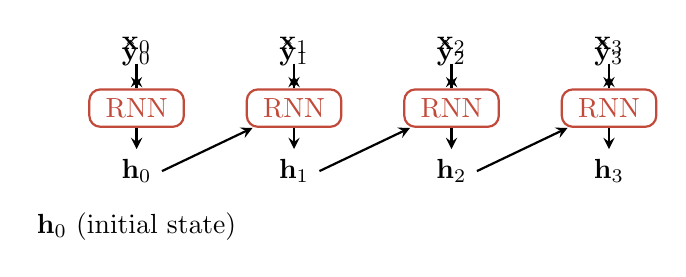
\begin{tikzpicture}[node distance=1cm, thick, >=stealth]
    \foreach \t in {0,1,2,3} {
        \pgfmathsetmacro{\prev}{\t-1}
        \node[draw, rectangle, rounded corners, wp-primary, minimum width=1.2cm] (cell\t) at (\t*2,0) {RNN};
        \node[above of=cell\t, node distance=0.8cm] (x\t) {$\mathbf{x}_\t$};
        \draw[->] (x\t) -- (cell\t);
        \node[below of=cell\t, node distance=0.8cm] (h\t) {$\mathbf{h}_\t$};
        \draw[->] (cell\t) -- (h\t);
        \node[above of=h\t, node distance=1.5cm] (y\t) {$\hat{\mathbf{y}}_\t$};
        \draw[->] (cell\t) -- (y\t);
        \ifnum\t>0
            \draw[->] (h\prev) -- (cell\t);
        \fi
    }
    \node at (0, -1.5) {$\mathbf{h}_0$ (initial state)};
\end{tikzpicture}
\caption{Unrolled RNN for $T=4$ time steps. The same weights $\mathbf{W}_{xh}, \mathbf{W}_{hh}, \mathbf{W}_{hy}$ are reused at every step.}
\label{fig:rnn_unrolled}
\end{figure}

\subsection{Forward Propagation}

Given an input sequence $\mathbf{x}_{1:T}$, forward propagation computes the hidden states and outputs sequentially:

\begin{algorithm}[h]
    \caption{Forward pass of an RNN}
    \begin{algorithmic}[1]
        \State $\mathbf{h}_0 \gets \mathbf{0}$ (or learned initial state)
        \For{$t = 1$ to $T$}
            \State $\mathbf{a}_t \gets \mathbf{W}_{xh}\mathbf{x}_t + \mathbf{W}_{hh}\mathbf{h}_{t-1} + \mathbf{b}_h$
            \State $\mathbf{h}_t \gets \phi_h(\mathbf{a}_t)$
            \State $\mathbf{o}_t \gets \mathbf{W}_{hy}\mathbf{h}_t + \mathbf{b}_y$
            \State $\hat{\mathbf{y}}_t \gets \phi_y(\mathbf{o}_t)$
        \EndFor
    \end{algorithmic}
\end{algorithm}

\section{Training RNNs: Backpropagation Through Time (BPTT)}

RNNs are trained by minimising a loss function that aggregates errors over all time steps. For a sequence with targets $\mathbf{y}_{1:T}$, the total loss is the sum of per‑time‑step losses:
\[
\mathcal{L}(\mathbf{y}_{1:T}, \hat{\mathbf{y}}_{1:T}) = \sum_{t=1}^{T} \ell(\mathbf{y}_t, \hat{\mathbf{y}}_t),
\]
where $\ell$ is a pointwise loss (e.g., cross‑entropy or squared error). Because the same parameters are shared across time, we must backpropagate gradients through the entire unrolled network. This procedure is called \textbf{backpropagation through time (BPTT)}.

\subsection{Gradient Computation}

Let $\theta$ denote any trainable parameter (e.g., $w_{ij}^{(xh)}$). The total derivative is
\[
\frac{\partial \mathcal{L}}{\partial \theta} = \sum_{t=1}^{T} \frac{\partial \ell_t}{\partial \theta},
\]
where $\ell_t$ is the loss at time $t$. For parameters that appear at every time step (like $\mathbf{W}_{hh}$), the contribution from each $t$ depends on all future time steps because the hidden state at time $t$ influences all subsequent losses.

We derive the gradients for $\mathbf{W}_{hh}$; similar reasoning applies to $\mathbf{W}_{xh}$, $\mathbf{b}_h$, $\mathbf{W}_{hy}$, $\mathbf{b}_y$.

\paragraph{Error Signals}
Define the error at the output of the RNN at time $t$ as:
\[
\boldsymbol{\delta}_t^{\text{out}} = \frac{\partial \ell_t}{\partial \mathbf{o}_t} = \nabla_{\hat{\mathbf{y}}_t} \ell_t \odot \phi_y'(\mathbf{o}_t).
\]
For the hidden layer, we need the sensitivity of the total future loss with respect to the pre‑activation $\mathbf{a}_t$. By the chain rule,
\[
\frac{\partial \mathcal{L}}{\partial \mathbf{a}_t} = \underbrace{\frac{\partial \ell_t}{\partial \mathbf{a}_t}}_{\text{immediate}} + \underbrace{\frac{\partial \mathcal{L}_{t+1:T}}{\partial \mathbf{a}_t}}_{\text{from future}}.
\]
The immediate contribution is $\frac{\partial \ell_t}{\partial \mathbf{a}_t} = \mathbf{W}_{hy}^{\mathsf{T}} \boldsymbol{\delta}_t^{\text{out}} \odot \phi_h'(\mathbf{a}_t)$.

The future contribution comes from the fact that $\mathbf{h}_t$ affects $\mathbf{a}_{t+1}$ via $\mathbf{W}_{hh}\mathbf{h}_t$. Hence,
\[
\frac{\partial \mathcal{L}_{t+1:T}}{\partial \mathbf{a}_t}
= \left( \frac{\partial \mathbf{a}_{t+1}}{\partial \mathbf{h}_t} \right)^{\mathsf{T}} \frac{\partial \mathcal{L}_{t+1:T}}{\partial \mathbf{a}_{t+1}}
= \mathbf{W}_{hh}^{\mathsf{T}} \boldsymbol{\delta}_{t+1} \odot \phi_h'(\mathbf{a}_t),
\]
where we define $\boldsymbol{\delta}_t = \frac{\partial \mathcal{L}}{\partial \mathbf{a}_t}$. Thus, the backward recurrence is:
\begin{align}
    \boldsymbol{\delta}_T &= \mathbf{W}_{hy}^{\mathsf{T}} \boldsymbol{\delta}_T^{\text{out}} \odot \phi_h'(\mathbf{a}_T), \\
    \boldsymbol{\delta}_t &= \left( \mathbf{W}_{hy}^{\mathsf{T}} \boldsymbol{\delta}_t^{\text{out}} + \mathbf{W}_{hh}^{\mathsf{T}} \boldsymbol{\delta}_{t+1} \right) \odot \phi_h'(\mathbf{a}_t), \quad t = T-1, \dots, 1.
\end{align}

\paragraph{Gradients with Respect to Weights}
Once the $\boldsymbol{\delta}_t$ are known, the gradients are:
\begin{align}
    \frac{\partial \mathcal{L}}{\partial \mathbf{W}_{hh}} &= \sum_{t=1}^{T} \boldsymbol{\delta}_t \, \mathbf{h}_{t-1}^{\mathsf{T}}, \\
    \frac{\partial \mathcal{L}}{\partial \mathbf{W}_{xh}} &= \sum_{t=1}^{T} \boldsymbol{\delta}_t \, \mathbf{x}_t^{\mathsf{T}}, \\
    \frac{\partial \mathcal{L}}{\partial \mathbf{b}_h} &= \sum_{t=1}^{T} \boldsymbol{\delta}_t, \\
    \frac{\partial \mathcal{L}}{\partial \mathbf{W}_{hy}} &= \sum_{t=1}^{T} \boldsymbol{\delta}_t^{\text{out}} \, \mathbf{h}_t^{\mathsf{T}}, \\
    \frac{\partial \mathcal{L}}{\partial \mathbf{b}_y} &= \sum_{t=1}^{T} \boldsymbol{\delta}_t^{\text{out}}.
\end{align}

These gradients are then used in any gradient‑based optimiser (SGD, Adam, etc.). The complete BPTT algorithm is summarised below.

\begin{algorithm}[h]
    \caption{Backpropagation Through Time (BPTT)}
    \begin{algorithmic}[1]
        \State Run forward pass to store $\mathbf{a}_t, \mathbf{h}_t, \mathbf{o}_t$ for $t=1,\dots,T$.
        \State Compute $\boldsymbol{\delta}_T^{\text{out}} = \nabla_{\hat{\mathbf{y}}_T}\ell_T \odot \phi_y'(\mathbf{o}_T)$.
        \State $\boldsymbol{\delta}_T = \mathbf{W}_{hy}^{\mathsf{T}} \boldsymbol{\delta}_T^{\text{out}} \odot \phi_h'(\mathbf{a}_T)$.
        \For{$t = T-1$ down to $1$}
            \State $\boldsymbol{\delta}_t^{\text{out}} = \nabla_{\hat{\mathbf{y}}_t}\ell_t \odot \phi_y'(\mathbf{o}_t)$
            \State $\boldsymbol{\delta}_t = \left( \mathbf{W}_{hy}^{\mathsf{T}} \boldsymbol{\delta}_t^{\text{out}} + \mathbf{W}_{hh}^{\mathsf{T}} \boldsymbol{\delta}_{t+1} \right) \odot \phi_h'(\mathbf{a}_t)$
        \EndFor
        \State Accumulate gradients for $\mathbf{W}_{hh}, \mathbf{W}_{xh}, \mathbf{b}_h, \mathbf{W}_{hy}, \mathbf{b}_y$ using the formulas above.
        \State Update parameters with gradient descent.
    \end{algorithmic}
\end{algorithm}

\subsection{Vanishing and Exploding Gradients}

A fundamental difficulty in training RNNs on long sequences is the problem of \textbf{vanishing} or \textbf{exploding gradients}. Observe that the recurrence for $\boldsymbol{\delta}_t$ involves multiplication by $\mathbf{W}_{hh}^{\mathsf{T}}$ and $\phi_h'(\mathbf{a}_t)$. Unrolling further, the gradient contains terms like $(\mathbf{W}_{hh}^{\mathsf{T}})^k \prod_{i=t+1}^{t+k} \phi_h'(\mathbf{a}_i)$. 

If the eigenvalues of $\mathbf{W}_{hh}$ are less than $1$ and the activation derivatives are also $<1$ (typical for sigmoid or $\tanh$), then long‑range gradients decay exponentially to zero (vanishing). Conversely, if eigenvalues exceed $1$, gradients explode. Vanishing gradients prevent the network from learning long‑range dependencies; exploding gradients make training numerically unstable.

\begin{thm}[Vanishing Gradients in RNNs]
    For a simple RNN with $\phi_h = \tanh$, let $\gamma = \max_i |\lambda_i(\mathbf{W}_{hh})|$ and $\rho = \max_z |\tanh'(z)| = 1$. If $\gamma < 1$, then the norm of the gradient contribution from time $t$ to time $t-k$ decays as $\mathcal{O}(\gamma^k)$.
\end{thm}

Solutions include:
\begin{itemize}
    \item Gradient clipping (for exploding gradients): rescale gradients if their norm exceeds a threshold.
    \item Careful weight initialisation (e.g., orthogonal initialisation).
    \item Gated architectures (LSTM, GRU) that allow gradients to flow more easily.
\end{itemize}

\section{Gated Recurrent Architectures}

To mitigate the vanishing gradient problem, more sophisticated RNN cells introduce \textbf{gates} that control the flow of information.

\subsection{Long Short‑Term Memory (LSTM)}

The LSTM, proposed by Hochreiter and Schmidhuber (1997), maintains a separate cell state $\mathbf{c}_t$ in addition to the hidden state $\mathbf{h}_t$. The cell state acts as a “conveyor belt” that can carry information over many steps. Three gates control access:

\begin{itemize}
    \item \textbf{Forget gate}: $\mathbf{f}_t = \sigma(\mathbf{W}_f [\mathbf{h}_{t-1}, \mathbf{x}_t] + \mathbf{b}_f)$
    \item \textbf{Input gate}: $\mathbf{i}_t = \sigma(\mathbf{W}_i [\mathbf{h}_{t-1}, \mathbf{x}_t] + \mathbf{b}_i)$
    \item \textbf{Output gate}: $\mathbf{o}_t = \sigma(\mathbf{W}_o [\mathbf{h}_{t-1}, \mathbf{x}_t] + \mathbf{b}_o)$
\end{itemize}

A candidate cell update is $\tilde{\mathbf{c}}_t = \tanh(\mathbf{W}_c [\mathbf{h}_{t-1}, \mathbf{x}_t] + \mathbf{b}_c)$. Then the cell state and hidden state are updated:
\begin{align}
    \mathbf{c}_t &= \mathbf{f}_t \odot \mathbf{c}_{t-1} + \mathbf{i}_t \odot \tilde{\mathbf{c}}_t, \\
    \mathbf{h}_t &= \mathbf{o}_t \odot \tanh(\mathbf{c}_t).
\end{align}

The forget gate allows the network to selectively erase the past; the input gate decides which new information to store; the output gate controls what is exposed as the hidden state.

\subsection{Gated Recurrent Unit (GRU)}

The GRU (Cho et al., 2014) simplifies the LSTM by combining the forget and input gates into a single \textbf{update gate} and merging the cell and hidden states. Its equations are:
\begin{align}
    \mathbf{z}_t &= \sigma(\mathbf{W}_z [\mathbf{h}_{t-1}, \mathbf{x}_t] + \mathbf{b}_z) \quad \text{(update gate)}, \\
    \mathbf{r}_t &= \sigma(\mathbf{W}_r [\mathbf{h}_{t-1}, \mathbf{x}_t] + \mathbf{b}_r) \quad \text{(reset gate)}, \\
    \tilde{\mathbf{h}}_t &= \tanh(\mathbf{W}_h [\mathbf{r}_t \odot \mathbf{h}_{t-1}, \mathbf{x}_t] + \mathbf{b}_h), \\
    \mathbf{h}_t &= (1 - \mathbf{z}_t) \odot \mathbf{h}_{t-1} + \mathbf{z}_t \odot \tilde{\mathbf{h}}_t.
\end{align}
GRUs have fewer parameters than LSTMs and often perform similarly.

\begin{marginfigure}
\centering
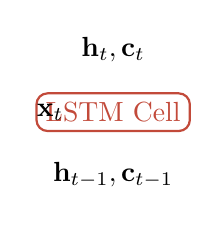
\begin{tikzpicture}[node distance=0.8cm, thick]
    \node[draw, rectangle, rounded corners, wp-primary] (lstm) {LSTM Cell};
    \node[above of=lstm] {$\mathbf{h}_t, \mathbf{c}_t$};
    \node[below of=lstm] {$\mathbf{h}_{t-1}, \mathbf{c}_{t-1}$};
    \node[left of=lstm] {$\mathbf{x}_t$};
\end{tikzpicture}
\caption{Schematic of an LSTM cell. The cell state $\mathbf{c}_t$ (not shown separately) flows through the top, modulated by gates.}
\end{marginfigure}

\subsection{Connection to Maximum Likelihood Estimation}

For sequence prediction (e.g., language modeling), the RNN defines a conditional probability distribution over the next token given the history:
\[
P(\mathbf{y}_t \mid \mathbf{x}_{1:t}, \mathbf{y}_{1:t-1}) = \text{softmax}(\mathbf{o}_t).
\]
The total likelihood of a sequence is $\prod_{t=1}^T P(\mathbf{y}_t \mid \text{history})$. Minimising the cross‑entropy loss is therefore equivalent to maximum likelihood estimation under the model.

\section{Practical Considerations and Extensions}

\begin{itemize}
    \item \textbf{Truncated BPTT}: For very long sequences, full BPTT is expensive. Truncated BPTT splits the sequence into blocks and only backpropagates a fixed number of steps ($k$) inside each block. This approximates the true gradient and is widely used.
    \item \textbf{Teacher forcing}: During training, the true previous target $\mathbf{y}_{t-1}$ (or a sample) is fed as input instead of the model’s own prediction. This speeds up training but may cause exposure bias.
    \item \textbf{Deep RNNs}: Stacking multiple RNN layers (each layer’s hidden state becomes input to the next layer) increases representational capacity.
    \item \textbf{Bidirectional RNNs}: Two RNNs process the sequence forward and backward, and their hidden states are concatenated. This provides context from both past and future, useful for sequence tagging.
\end{itemize}

\begin{algorithm}[h]
    \caption{Truncated BPTT (with block size $k$)}
    \begin{algorithmic}[1]
        \State Initialise $\mathbf{h}_0$.
        \For{each block $b$ of $k$ consecutive time steps}
            \State Run forward pass for $k$ steps, storing intermediate values.
            \State Compute loss for the block.
            \State Backpropagate gradients only through the $k$ steps (do not propagate beyond the block start).
            \State Update parameters.
            \State Carry over $\mathbf{h}_{b \cdot k}$ as initial state for the next block.
        \EndFor
    \end{algorithmic}
\end{algorithm}

\section{Summary}

Recurrent Neural Networks provide a principled framework for modeling sequential data by maintaining an internal state that evolves over time. The training procedure, backpropagation through time, is a direct extension of the backpropagation algorithm for feedforward networks but must handle weight sharing across time. The vanishing and exploding gradient problems are inherent to simple RNNs; gated architectures (LSTM, GRU) are the standard solution. These models form the basis of modern sequence‑to‑sequence learning, machine translation, speech recognition, and many other applications.

The mathematical tools developed in earlier chapters – probability, MLE, gradient descent, and information theory – all play a role in understanding and training RNNs. The next logical step is to explore attention mechanisms and transformers, which have largely replaced RNNs in many domains but still rely on the same foundational concepts.

\end{document}